GUI składa się dwóch sekcji: panel sterowania, wyświetlacz. Realizują one następujące funkcje:
\begin{itemize}
    \item \textbf{Panel sterowania:} Dostarczenie interfejsu do integracji użytkownika z silnikiem detekcji obiektów, w tym możliwość zmiany parametrów detektora obrazu oraz ustawienie źródła wideo. Zarządzanie wyświetlaniem klatek obrazu -- wywołanie funkcji odpowiedzialnej za wyświetlenie klatki.
    \item \textbf{Wyświetlacz: } Wyświetlanie klatek obrazu.
\end{itemize}

Panel sterowania nie jest skomplikowany, dlatego też nie wymaga użycia złożonej technologii. Z kolei wyświetlacz wymaga tylko jednej funkcji, natomiast musi być ona jak najlepiej zomptymalizowana. Biorąc pod uwage te czynniki zdecydowano się na użycie dwóch różnych technologii i zintegrowanie ich w jeden graficzny interfejs użytkownika.

Za panel sterowania, odpowiada moduł tkinter -- GUI z biblioteki standardowej języka Python. Jest to dobrze udokumentowane i lekkie rozwiązanie. W przypadku wyświetlania, ponownie zdecydowano się na użycie bilbioteki OpenCV, a dokładniej funkcji \emph{cv2.imshow()}. Jest to funkcja specjalnie zoptymalizowana pod wyświetlanie oraz, tak jak jak to zostało wspomniane, jedyna konieczna do wyświetlenia obrazu.
Zrezygnowano z użycia tkinter jako wyświetlacza, ponieważ nie jest on zoptymalizowany pod wyświetlanie klatek z dużą częstotliwością. 

Dokumentacja do modułu tkinter zawiera się w dokumentacji języka Python \cite{Python_docs}.

\begin{figure}[H]
    \centering
    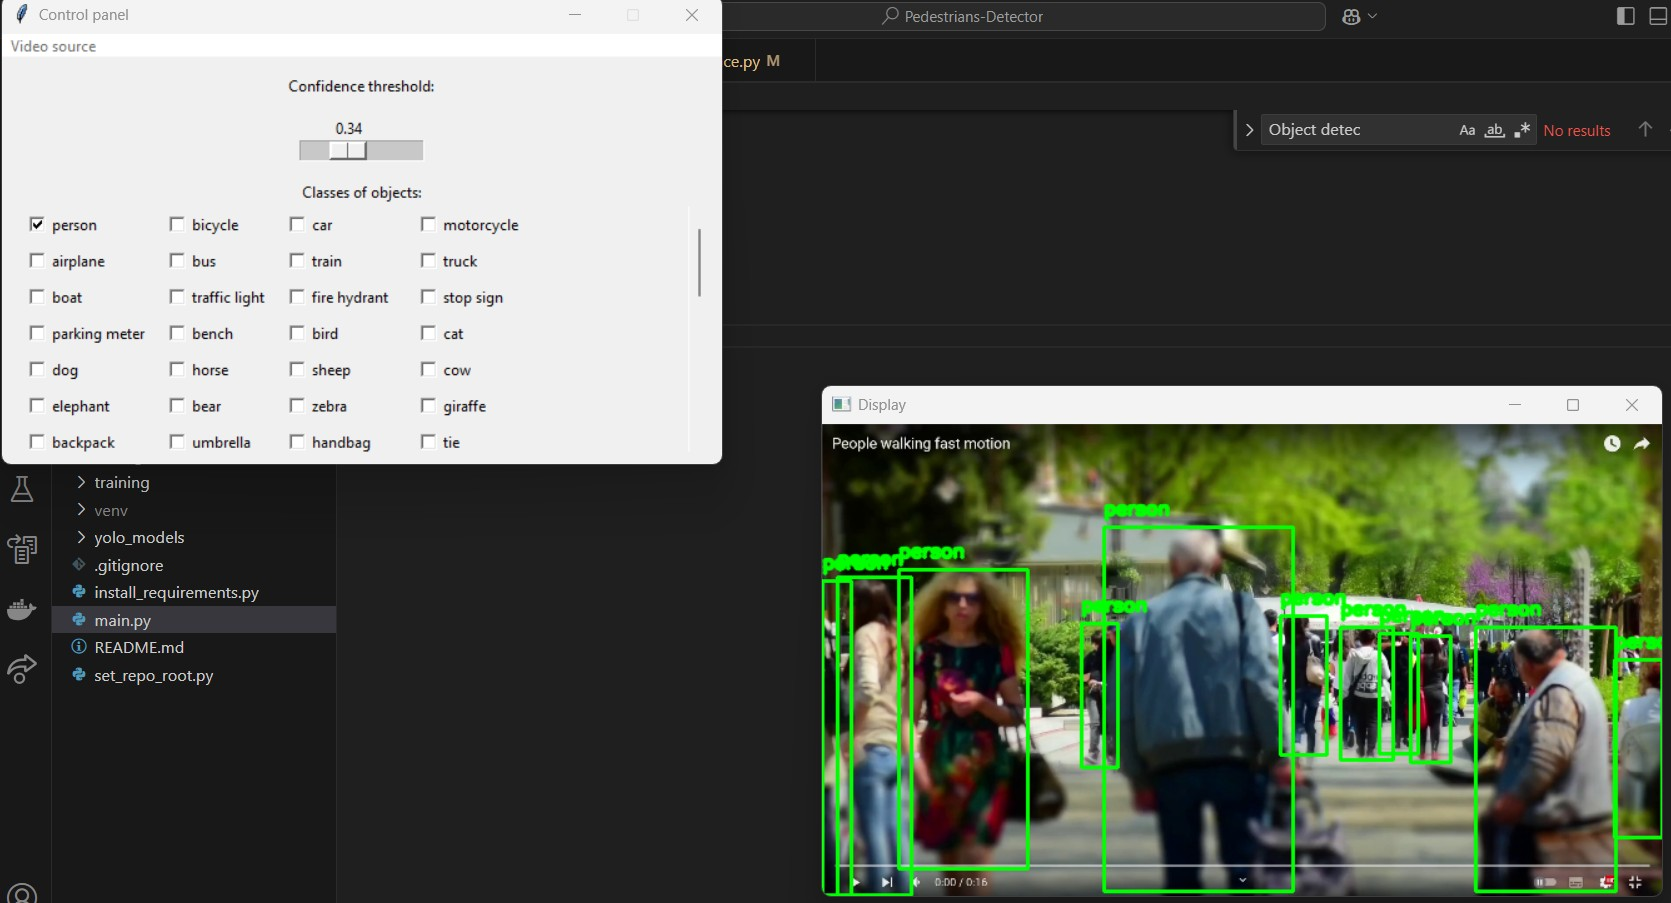
\includegraphics[width=\linewidth]{r_technologie/GUI_assets/mockup.jpg}
    \caption{Wygląd GUI w projekcie: panel sterowania -- w lewym górnym rogu, wyświetlacz -- w prawym dolnym rogu}
    \label{fig:technologies-GUI}
\end{figure}